% Options for packages loaded elsewhere
% Options for packages loaded elsewhere
\PassOptionsToPackage{unicode}{hyperref}
\PassOptionsToPackage{hyphens}{url}
\PassOptionsToPackage{dvipsnames,svgnames,x11names}{xcolor}
%
\documentclass[
  letterpaper,
  DIV=11,
  numbers=noendperiod]{scrreprt}
\usepackage{xcolor}
\usepackage{amsmath,amssymb}
\setcounter{secnumdepth}{5}
\usepackage{iftex}
\ifPDFTeX
  \usepackage[T1]{fontenc}
  \usepackage[utf8]{inputenc}
  \usepackage{textcomp} % provide euro and other symbols
\else % if luatex or xetex
  \usepackage{unicode-math} % this also loads fontspec
  \defaultfontfeatures{Scale=MatchLowercase}
  \defaultfontfeatures[\rmfamily]{Ligatures=TeX,Scale=1}
\fi
\usepackage{lmodern}
\ifPDFTeX\else
  % xetex/luatex font selection
\fi
% Use upquote if available, for straight quotes in verbatim environments
\IfFileExists{upquote.sty}{\usepackage{upquote}}{}
\IfFileExists{microtype.sty}{% use microtype if available
  \usepackage[]{microtype}
  \UseMicrotypeSet[protrusion]{basicmath} % disable protrusion for tt fonts
}{}
\makeatletter
\@ifundefined{KOMAClassName}{% if non-KOMA class
  \IfFileExists{parskip.sty}{%
    \usepackage{parskip}
  }{% else
    \setlength{\parindent}{0pt}
    \setlength{\parskip}{6pt plus 2pt minus 1pt}}
}{% if KOMA class
  \KOMAoptions{parskip=half}}
\makeatother
% Make \paragraph and \subparagraph free-standing
\makeatletter
\ifx\paragraph\undefined\else
  \let\oldparagraph\paragraph
  \renewcommand{\paragraph}{
    \@ifstar
      \xxxParagraphStar
      \xxxParagraphNoStar
  }
  \newcommand{\xxxParagraphStar}[1]{\oldparagraph*{#1}\mbox{}}
  \newcommand{\xxxParagraphNoStar}[1]{\oldparagraph{#1}\mbox{}}
\fi
\ifx\subparagraph\undefined\else
  \let\oldsubparagraph\subparagraph
  \renewcommand{\subparagraph}{
    \@ifstar
      \xxxSubParagraphStar
      \xxxSubParagraphNoStar
  }
  \newcommand{\xxxSubParagraphStar}[1]{\oldsubparagraph*{#1}\mbox{}}
  \newcommand{\xxxSubParagraphNoStar}[1]{\oldsubparagraph{#1}\mbox{}}
\fi
\makeatother

\usepackage{color}
\usepackage{fancyvrb}
\newcommand{\VerbBar}{|}
\newcommand{\VERB}{\Verb[commandchars=\\\{\}]}
\DefineVerbatimEnvironment{Highlighting}{Verbatim}{commandchars=\\\{\}}
% Add ',fontsize=\small' for more characters per line
\usepackage{framed}
\definecolor{shadecolor}{RGB}{241,243,245}
\newenvironment{Shaded}{\begin{snugshade}}{\end{snugshade}}
\newcommand{\AlertTok}[1]{\textcolor[rgb]{0.68,0.00,0.00}{#1}}
\newcommand{\AnnotationTok}[1]{\textcolor[rgb]{0.37,0.37,0.37}{#1}}
\newcommand{\AttributeTok}[1]{\textcolor[rgb]{0.40,0.45,0.13}{#1}}
\newcommand{\BaseNTok}[1]{\textcolor[rgb]{0.68,0.00,0.00}{#1}}
\newcommand{\BuiltInTok}[1]{\textcolor[rgb]{0.00,0.23,0.31}{#1}}
\newcommand{\CharTok}[1]{\textcolor[rgb]{0.13,0.47,0.30}{#1}}
\newcommand{\CommentTok}[1]{\textcolor[rgb]{0.37,0.37,0.37}{#1}}
\newcommand{\CommentVarTok}[1]{\textcolor[rgb]{0.37,0.37,0.37}{\textit{#1}}}
\newcommand{\ConstantTok}[1]{\textcolor[rgb]{0.56,0.35,0.01}{#1}}
\newcommand{\ControlFlowTok}[1]{\textcolor[rgb]{0.00,0.23,0.31}{\textbf{#1}}}
\newcommand{\DataTypeTok}[1]{\textcolor[rgb]{0.68,0.00,0.00}{#1}}
\newcommand{\DecValTok}[1]{\textcolor[rgb]{0.68,0.00,0.00}{#1}}
\newcommand{\DocumentationTok}[1]{\textcolor[rgb]{0.37,0.37,0.37}{\textit{#1}}}
\newcommand{\ErrorTok}[1]{\textcolor[rgb]{0.68,0.00,0.00}{#1}}
\newcommand{\ExtensionTok}[1]{\textcolor[rgb]{0.00,0.23,0.31}{#1}}
\newcommand{\FloatTok}[1]{\textcolor[rgb]{0.68,0.00,0.00}{#1}}
\newcommand{\FunctionTok}[1]{\textcolor[rgb]{0.28,0.35,0.67}{#1}}
\newcommand{\ImportTok}[1]{\textcolor[rgb]{0.00,0.46,0.62}{#1}}
\newcommand{\InformationTok}[1]{\textcolor[rgb]{0.37,0.37,0.37}{#1}}
\newcommand{\KeywordTok}[1]{\textcolor[rgb]{0.00,0.23,0.31}{\textbf{#1}}}
\newcommand{\NormalTok}[1]{\textcolor[rgb]{0.00,0.23,0.31}{#1}}
\newcommand{\OperatorTok}[1]{\textcolor[rgb]{0.37,0.37,0.37}{#1}}
\newcommand{\OtherTok}[1]{\textcolor[rgb]{0.00,0.23,0.31}{#1}}
\newcommand{\PreprocessorTok}[1]{\textcolor[rgb]{0.68,0.00,0.00}{#1}}
\newcommand{\RegionMarkerTok}[1]{\textcolor[rgb]{0.00,0.23,0.31}{#1}}
\newcommand{\SpecialCharTok}[1]{\textcolor[rgb]{0.37,0.37,0.37}{#1}}
\newcommand{\SpecialStringTok}[1]{\textcolor[rgb]{0.13,0.47,0.30}{#1}}
\newcommand{\StringTok}[1]{\textcolor[rgb]{0.13,0.47,0.30}{#1}}
\newcommand{\VariableTok}[1]{\textcolor[rgb]{0.07,0.07,0.07}{#1}}
\newcommand{\VerbatimStringTok}[1]{\textcolor[rgb]{0.13,0.47,0.30}{#1}}
\newcommand{\WarningTok}[1]{\textcolor[rgb]{0.37,0.37,0.37}{\textit{#1}}}

\usepackage{longtable,booktabs,array}
\usepackage{calc} % for calculating minipage widths
% Correct order of tables after \paragraph or \subparagraph
\usepackage{etoolbox}
\makeatletter
\patchcmd\longtable{\par}{\if@noskipsec\mbox{}\fi\par}{}{}
\makeatother
% Allow footnotes in longtable head/foot
\IfFileExists{footnotehyper.sty}{\usepackage{footnotehyper}}{\usepackage{footnote}}
\makesavenoteenv{longtable}
\usepackage{graphicx}
\makeatletter
\newsavebox\pandoc@box
\newcommand*\pandocbounded[1]{% scales image to fit in text height/width
  \sbox\pandoc@box{#1}%
  \Gscale@div\@tempa{\textheight}{\dimexpr\ht\pandoc@box+\dp\pandoc@box\relax}%
  \Gscale@div\@tempb{\linewidth}{\wd\pandoc@box}%
  \ifdim\@tempb\p@<\@tempa\p@\let\@tempa\@tempb\fi% select the smaller of both
  \ifdim\@tempa\p@<\p@\scalebox{\@tempa}{\usebox\pandoc@box}%
  \else\usebox{\pandoc@box}%
  \fi%
}
% Set default figure placement to htbp
\def\fps@figure{htbp}
\makeatother





\setlength{\emergencystretch}{3em} % prevent overfull lines

\providecommand{\tightlist}{%
  \setlength{\itemsep}{0pt}\setlength{\parskip}{0pt}}



 


\KOMAoption{captions}{tableheading}
\makeatletter
\@ifpackageloaded{bookmark}{}{\usepackage{bookmark}}
\makeatother
\makeatletter
\@ifpackageloaded{caption}{}{\usepackage{caption}}
\AtBeginDocument{%
\ifdefined\contentsname
  \renewcommand*\contentsname{Table of contents}
\else
  \newcommand\contentsname{Table of contents}
\fi
\ifdefined\listfigurename
  \renewcommand*\listfigurename{List of Figures}
\else
  \newcommand\listfigurename{List of Figures}
\fi
\ifdefined\listtablename
  \renewcommand*\listtablename{List of Tables}
\else
  \newcommand\listtablename{List of Tables}
\fi
\ifdefined\figurename
  \renewcommand*\figurename{Figure}
\else
  \newcommand\figurename{Figure}
\fi
\ifdefined\tablename
  \renewcommand*\tablename{Table}
\else
  \newcommand\tablename{Table}
\fi
}
\@ifpackageloaded{float}{}{\usepackage{float}}
\floatstyle{ruled}
\@ifundefined{c@chapter}{\newfloat{codelisting}{h}{lop}}{\newfloat{codelisting}{h}{lop}[chapter]}
\floatname{codelisting}{Listing}
\newcommand*\listoflistings{\listof{codelisting}{List of Listings}}
\makeatother
\makeatletter
\makeatother
\makeatletter
\@ifpackageloaded{caption}{}{\usepackage{caption}}
\@ifpackageloaded{subcaption}{}{\usepackage{subcaption}}
\makeatother
\usepackage{bookmark}
\IfFileExists{xurl.sty}{\usepackage{xurl}}{} % add URL line breaks if available
\urlstyle{same}
\hypersetup{
  pdftitle={合成菌群文献复现项目},
  pdfauthor={liuhaodong,luanyehui},
  colorlinks=true,
  linkcolor={blue},
  filecolor={Maroon},
  citecolor={Blue},
  urlcolor={Blue},
  pdfcreator={LaTeX via pandoc}}


\title{合成菌群文献复现项目}
\author{liuhaodong,luanyehui}
\date{}
\begin{document}
\maketitle

\renewcommand*\contentsname{Table of contents}
{
\hypersetup{linkcolor=}
\setcounter{tocdepth}{2}
\tableofcontents
}

\bookmarksetup{startatroot}

\chapter*{Preface}\label{preface}
\addcontentsline{toc}{chapter}{Preface}

\markboth{Preface}{Preface}

This is a Quarto book.

To learn more about Quarto books visit
\url{https://quarto.org/docs/books}.

\bookmarksetup{startatroot}

\chapter{核心结果：微生物群落的时间序列变化}\label{ux6838ux5fc3ux7ed3ux679cux5faeux751fux7269ux7fa4ux843dux7684ux65f6ux95f4ux5e8fux5217ux53d8ux5316}

\section{1.
研究背景与数据准备}\label{ux7814ux7a76ux80ccux666fux4e0eux6570ux636eux51c6ux5907}

为了探究微生物群落结构随时间的演替规律，我们首先复现了原论文图 1A
的群落时间序列分析。

首先，加载数据处理和可视化所需的核心工具包
\texttt{tidyverse}（这也能解决我们环境中未识别基础函数的警告）。接着，我们读取
ASV（扩增子变异序列）的分类学元数据。

\begin{Shaded}
\begin{Highlighting}[]
\CommentTok{\# 加载核心包}
\FunctionTok{library}\NormalTok{(tidyverse)}

\CommentTok{\# 读取元数据：提供序列 ID 与较高分类学级别的映射关系}
\NormalTok{taxa\_info }\OtherTok{\textless{}{-}} \FunctionTok{read.csv}\NormalTok{(}\StringTok{"../data/taxa\_information.csv"}\NormalTok{)}
\end{Highlighting}
\end{Shaded}

\section{2.
数据清洗与分类学聚合}\label{ux6570ux636eux6e05ux6d17ux4e0eux5206ux7c7bux5b66ux805aux5408}

原始测序数据通常是宽表格式且非常庞杂。为了能够进行宏观的群落结构分析，我们需要将其转换为时间序列长表，并将底层的
ASV 丰度聚合到更高的分类学层级（如硅藻、甲藻等）。

\begin{Shaded}
\begin{Highlighting}[]
\CommentTok{\# 读取时间序列丰度数据并进行预处理}
\NormalTok{data }\OtherTok{\textless{}{-}} \FunctionTok{read.csv}\NormalTok{(}\StringTok{"../data/data\_sequences\_0.1\_rel\_ab\_0.5\_occ\_binned\_4\_days\_with\_temperature.csv"}\NormalTok{) }\SpecialCharTok{\%\textgreater{}\%}
  \CommentTok{\# 宽表转长表，适应时间序列绘图}
  \FunctionTok{gather}\NormalTok{(}\SpecialCharTok{{-}}\NormalTok{date, }\AttributeTok{key =} \StringTok{"variable"}\NormalTok{, }\AttributeTok{value =} \StringTok{"value"}\NormalTok{) }\SpecialCharTok{\%\textgreater{}\%}
  \CommentTok{\# 匹配分类学标签}
  \FunctionTok{left\_join}\NormalTok{(taxa\_info, }\AttributeTok{by =} \FunctionTok{c}\NormalTok{(}\StringTok{"variable"} \OtherTok{=} \StringTok{"sequence\_ID"}\NormalTok{)) }\SpecialCharTok{\%\textgreater{}\%}
  \CommentTok{\# 质控：剔除无法进行分类学鉴定的序列}
  \FunctionTok{filter}\NormalTok{(}\SpecialCharTok{!}\FunctionTok{is.na}\NormalTok{(domain)) }\SpecialCharTok{\%\textgreater{}\%} 
  \CommentTok{\# 将单个 ASV 的相对丰度聚合到各自的高级分类群中}
  \FunctionTok{group\_by}\NormalTok{(date, group, domain) }\SpecialCharTok{\%\textgreater{}\%}
  \FunctionTok{summarise}\NormalTok{(}\AttributeTok{rel\_ab =} \FunctionTok{sum}\NormalTok{(value, }\AttributeTok{na.rm =} \ConstantTok{TRUE}\NormalTok{), }\AttributeTok{.groups =} \StringTok{"drop"}\NormalTok{)}
\end{Highlighting}
\end{Shaded}

\section{3.
图表属性配置与总丰度计算}\label{ux56feux8868ux5c5eux6027ux914dux7f6eux4e0eux603bux4e30ux5ea6ux8ba1ux7b97}

为了让图表具有良好的可读性，我们提取了原作者预设的颜色配置，并强制按照丰度和域（domain）进行排序。同时，我们计算了群落的``总丰度''，并将其标准化到
0-1 之间，以便在图中作为次坐标轴（折线）展示。

\begin{Shaded}
\begin{Highlighting}[]
\NormalTok{plotting\_attributes }\OtherTok{\textless{}{-}}\NormalTok{ taxa\_info }\SpecialCharTok{\%\textgreater{}\%}
  \FunctionTok{select}\NormalTok{(group, domain, rel\_ab\_mean, color) }\SpecialCharTok{\%\textgreater{}\%}
  \FunctionTok{filter}\NormalTok{(}\SpecialCharTok{!}\FunctionTok{is.na}\NormalTok{(domain)) }\SpecialCharTok{\%\textgreater{}\%} 
  \FunctionTok{group\_by}\NormalTok{(group, domain, color) }\SpecialCharTok{\%\textgreater{}\%}
  \FunctionTok{summarise}\NormalTok{(}\AttributeTok{rel\_ab =} \FunctionTok{sum}\NormalTok{(rel\_ab\_mean, }\AttributeTok{na.rm =} \ConstantTok{TRUE}\NormalTok{), }\AttributeTok{.groups =} \StringTok{"drop"}\NormalTok{) }\SpecialCharTok{\%\textgreater{}\%}
  \FunctionTok{arrange}\NormalTok{(domain, rel\_ab)}

\NormalTok{plot\_data }\OtherTok{\textless{}{-}}\NormalTok{ data }\SpecialCharTok{\%\textgreater{}\%}
  \FunctionTok{mutate}\NormalTok{(}\AttributeTok{group =} \FunctionTok{factor}\NormalTok{(group, }\AttributeTok{levels =} \FunctionTok{pull}\NormalTok{(plotting\_attributes, }\StringTok{"group"}\NormalTok{)))}

\NormalTok{scale\_values }\OtherTok{\textless{}{-}} \ControlFlowTok{function}\NormalTok{(x)\{(x }\SpecialCharTok{{-}} \FunctionTok{min}\NormalTok{(x, }\AttributeTok{na.rm =} \ConstantTok{TRUE}\NormalTok{)) }\SpecialCharTok{/}\NormalTok{ (}\FunctionTok{max}\NormalTok{(x, }\AttributeTok{na.rm =} \ConstantTok{TRUE}\NormalTok{) }\SpecialCharTok{{-}} \FunctionTok{min}\NormalTok{(x, }\AttributeTok{na.rm =} \ConstantTok{TRUE}\NormalTok{))\} }

\NormalTok{total\_abundance\_scaled }\OtherTok{\textless{}{-}} \FunctionTok{ungroup}\NormalTok{(data) }\SpecialCharTok{\%\textgreater{}\%}
  \FunctionTok{group\_by}\NormalTok{(date) }\SpecialCharTok{\%\textgreater{}\%}
  \FunctionTok{summarise}\NormalTok{(}\AttributeTok{rel\_ab =} \FunctionTok{sum}\NormalTok{(rel\_ab), }\AttributeTok{.groups =} \StringTok{"drop"}\NormalTok{) }\SpecialCharTok{\%\textgreater{}\%} 
  \FunctionTok{mutate}\NormalTok{(}\AttributeTok{rel\_ab =} \FunctionTok{ifelse}\NormalTok{(rel\_ab }\SpecialCharTok{==} \DecValTok{0}\NormalTok{, }\ConstantTok{NA}\NormalTok{, rel\_ab)) }\SpecialCharTok{\%\textgreater{}\%} 
  \FunctionTok{mutate}\NormalTok{(}\AttributeTok{rel\_ab\_scaled =} \FunctionTok{scale\_values}\NormalTok{(rel\_ab))}
\end{Highlighting}
\end{Shaded}

\section{4.
核心结果可视化与解读\ldots{}}\label{ux6838ux5fc3ux7ed3ux679cux53efux89c6ux5316ux4e0eux89e3ux8bfb}

\begin{Shaded}
\begin{Highlighting}[]
\FunctionTok{ggplot}\NormalTok{(plot\_data, }\FunctionTok{aes}\NormalTok{(}\AttributeTok{y =}\NormalTok{ rel\_ab, }\AttributeTok{x =} \FunctionTok{date}\NormalTok{(date))) }\SpecialCharTok{+}
  \FunctionTok{geom\_bar}\NormalTok{(}\AttributeTok{stat =} \StringTok{"identity"}\NormalTok{, }\FunctionTok{aes}\NormalTok{(}\AttributeTok{color =}\NormalTok{ group, }\AttributeTok{fill =}\NormalTok{ group), }\AttributeTok{position =} \StringTok{"fill"}\NormalTok{) }\SpecialCharTok{+}
  \FunctionTok{scale\_color\_manual}\NormalTok{(}\AttributeTok{values =} \FunctionTok{pull}\NormalTok{(plotting\_attributes, }\StringTok{"color"}\NormalTok{), }\AttributeTok{name =} \StringTok{""}\NormalTok{) }\SpecialCharTok{+}
  \FunctionTok{scale\_fill\_manual}\NormalTok{(}\AttributeTok{values =} \FunctionTok{pull}\NormalTok{(plotting\_attributes, }\StringTok{"color"}\NormalTok{), }\AttributeTok{name =} \StringTok{""}\NormalTok{) }\SpecialCharTok{+}
  \FunctionTok{theme\_classic}\NormalTok{() }\SpecialCharTok{+}
  \FunctionTok{ylab}\NormalTok{(}\StringTok{"Community composition (scaled)"}\NormalTok{) }\SpecialCharTok{+}
  \FunctionTok{xlab}\NormalTok{(}\StringTok{"Time"}\NormalTok{) }\SpecialCharTok{+}
  \FunctionTok{theme}\NormalTok{(}\AttributeTok{legend.position =} \StringTok{"top"}\NormalTok{, }
        \AttributeTok{text =} \FunctionTok{element\_text}\NormalTok{(}\AttributeTok{size =} \DecValTok{12}\NormalTok{), }
        \AttributeTok{legend.text =} \FunctionTok{element\_text}\NormalTok{(}\AttributeTok{size =} \DecValTok{8}\NormalTok{), }
        \AttributeTok{legend.key.size =} \FunctionTok{unit}\NormalTok{(}\FloatTok{0.3}\NormalTok{, }\StringTok{"cm"}\NormalTok{)) }\SpecialCharTok{+} 
  \FunctionTok{scale\_x\_date}\NormalTok{(}\AttributeTok{date\_breaks =} \StringTok{"1 year"}\NormalTok{, }\AttributeTok{date\_labels =} \StringTok{"\%Y"}\NormalTok{, }\AttributeTok{expand =} \FunctionTok{c}\NormalTok{(}\DecValTok{0}\NormalTok{, }\DecValTok{0}\NormalTok{)) }\SpecialCharTok{+}
  \FunctionTok{scale\_y\_continuous}\NormalTok{(}\AttributeTok{expand =} \FunctionTok{c}\NormalTok{(}\DecValTok{0}\NormalTok{, }\DecValTok{0}\NormalTok{), }
                     \AttributeTok{sec.axis =} \FunctionTok{sec\_axis}\NormalTok{(}\SpecialCharTok{\textasciitilde{}}\NormalTok{. }\SpecialCharTok{*} \DecValTok{1}\NormalTok{, }\AttributeTok{name =} \StringTok{"Total abundance (scaled)"}\NormalTok{, }\AttributeTok{breaks =} \FunctionTok{seq}\NormalTok{(}\DecValTok{0}\NormalTok{, }\DecValTok{1}\NormalTok{, }\FloatTok{0.2}\NormalTok{)), }
                     \AttributeTok{breaks =} \FunctionTok{seq}\NormalTok{(}\DecValTok{0}\NormalTok{, }\DecValTok{1}\NormalTok{, }\FloatTok{0.2}\NormalTok{)) }\SpecialCharTok{+}
  \FunctionTok{geom\_line}\NormalTok{(}\AttributeTok{data =}\NormalTok{ total\_abundance\_scaled, }\FunctionTok{aes}\NormalTok{(}\AttributeTok{y =}\NormalTok{ rel\_ab\_scaled), }\AttributeTok{color =} \StringTok{"white"}\NormalTok{, }\AttributeTok{linewidth =} \FloatTok{0.6}\NormalTok{) }\SpecialCharTok{+}
  \FunctionTok{guides}\NormalTok{(}\AttributeTok{colour =} \FunctionTok{guide\_legend}\NormalTok{(}\AttributeTok{nrow =} \DecValTok{2}\NormalTok{), }\AttributeTok{fill =} \FunctionTok{guide\_legend}\NormalTok{(}\AttributeTok{nrow =} \DecValTok{2}\NormalTok{))}

\FunctionTok{ggsave}\NormalTok{(}\StringTok{"../plots/Fig\_1A\_microbial\_community\_time\_series.pdf"}\NormalTok{, }\AttributeTok{width =} \DecValTok{12}\NormalTok{, }\AttributeTok{height =} \FloatTok{3.5}\NormalTok{)}
\end{Highlighting}
\end{Shaded}

\begin{figure}[H]

\centering{

\pandocbounded{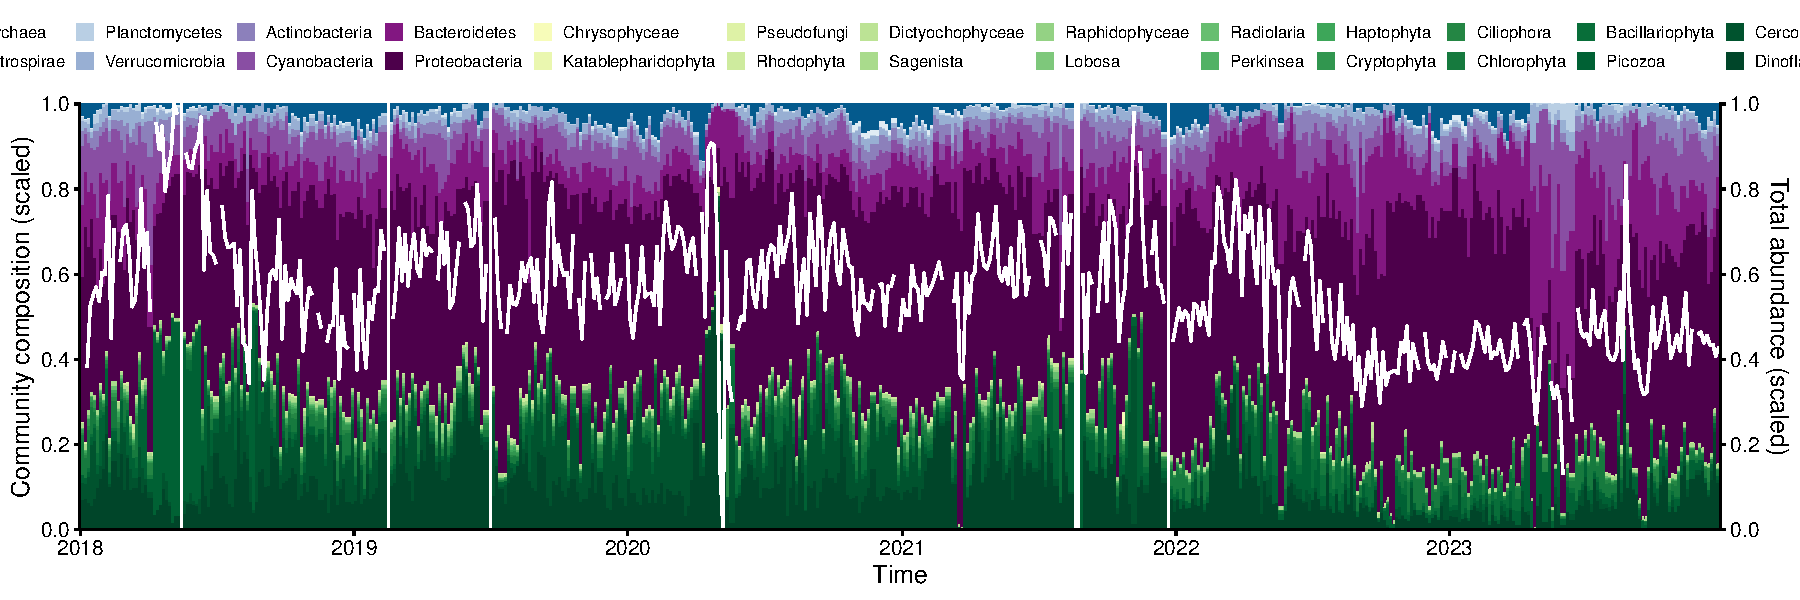
\includegraphics[keepaspectratio]{01-community-timeseries_files/figure-pdf/fig-community-composition-1.pdf}}

}

\caption{\label{fig-community-composition}图1：微生物群落组成与总丰度的时间序列变化}

\end{figure}%

\section{5.
环境驱动力分析：温度的时间序列}\label{ux73afux5883ux9a71ux52a8ux529bux5206ux6790ux6e29ux5ea6ux7684ux65f6ux95f4ux5e8fux5217}

在跳过极其消耗算力的微生物内部互作计算后，我们直接探索外部环境因子（如温度）对群落演替的潜在影响。原论文的图
4
探讨了这种温度依赖性。由于我们本地的数据集已经包含了水温记录，我们可以直接提取并将其可视化。

\begin{Shaded}
\begin{Highlighting}[]
\CommentTok{\# 重新读取原始宽表数据并专门提取温度列}
\NormalTok{raw\_data }\OtherTok{\textless{}{-}} \FunctionTok{read.csv}\NormalTok{(}\StringTok{"../data/data\_sequences\_0.1\_rel\_ab\_0.5\_occ\_binned\_4\_days\_with\_temperature.csv"}\NormalTok{)}

\CommentTok{\# 整理环境数据（剔除多余的物种丰度列，保留时间和温度）}
\NormalTok{env\_data }\OtherTok{\textless{}{-}}\NormalTok{ raw\_data }\SpecialCharTok{\%\textgreater{}\%}
  \FunctionTok{select}\NormalTok{(date, temperature) }\SpecialCharTok{\%\textgreater{}\%}
  \CommentTok{\# 确保日期列被 R 语言正确识别为时间格式}
  \FunctionTok{mutate}\NormalTok{(}\AttributeTok{date =} \FunctionTok{as.Date}\NormalTok{(date))}

\CommentTok{\# 绘制温度变化折线图}
\FunctionTok{ggplot}\NormalTok{(env\_data, }\FunctionTok{aes}\NormalTok{(}\AttributeTok{x =}\NormalTok{ date, }\AttributeTok{y =}\NormalTok{ temperature)) }\SpecialCharTok{+}
  \CommentTok{\# 绘制温度主线（橙红色）}
  \FunctionTok{geom\_line}\NormalTok{(}\AttributeTok{color =} \StringTok{"\#d95f02"}\NormalTok{, }\AttributeTok{linewidth =} \FloatTok{0.8}\NormalTok{) }\SpecialCharTok{+}
  \CommentTok{\# 添加一条平滑的长期趋势线（黑色虚线）}
  \FunctionTok{geom\_smooth}\NormalTok{(}\AttributeTok{method =} \StringTok{"loess"}\NormalTok{, }\AttributeTok{color =} \StringTok{"black"}\NormalTok{, }\AttributeTok{linetype =} \StringTok{"dashed"}\NormalTok{, }\AttributeTok{se =} \ConstantTok{FALSE}\NormalTok{) }\SpecialCharTok{+}
  \FunctionTok{theme\_classic}\NormalTok{() }\SpecialCharTok{+}
  \FunctionTok{labs}\NormalTok{(}\AttributeTok{y =} \StringTok{"Temperature (°C)"}\NormalTok{, }\AttributeTok{x =} \StringTok{"Time"}\NormalTok{) }\SpecialCharTok{+}
  \FunctionTok{scale\_x\_date}\NormalTok{(}\AttributeTok{date\_breaks =} \StringTok{"1 year"}\NormalTok{, }\AttributeTok{date\_labels =} \StringTok{"\%Y"}\NormalTok{, }\AttributeTok{expand =} \FunctionTok{c}\NormalTok{(}\DecValTok{0}\NormalTok{, }\DecValTok{0}\NormalTok{)) }\SpecialCharTok{+}
  \FunctionTok{theme}\NormalTok{(}\AttributeTok{text =} \FunctionTok{element\_text}\NormalTok{(}\AttributeTok{size =} \DecValTok{12}\NormalTok{))}

\CommentTok{\# 保存图片到 plots 文件夹}
\FunctionTok{ggsave}\NormalTok{(}\StringTok{"../plots/Fig\_4A\_Temperature\_series.pdf"}\NormalTok{, }\AttributeTok{width =} \DecValTok{10}\NormalTok{, }\AttributeTok{height =} \DecValTok{3}\NormalTok{)}
\end{Highlighting}
\end{Shaded}

\begin{figure}[H]

\centering{

\pandocbounded{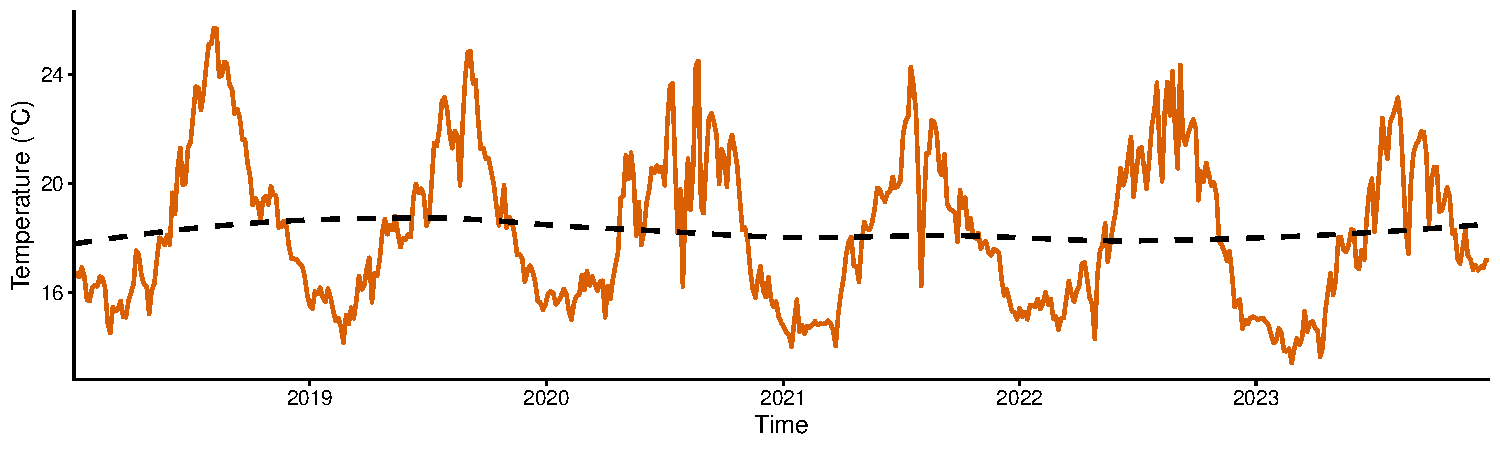
\includegraphics[keepaspectratio]{01-community-timeseries_files/figure-pdf/fig-temperature-dynamics-1.pdf}}

}

\caption{\label{fig-temperature-dynamics}图2：采样期间水温的时间序列与季节性波动}

\end{figure}%

\section{6.
微生物互作强度的温度依赖性（数据准备）}\label{ux5faeux751fux7269ux4e92ux4f5cux5f3aux5ea6ux7684ux6e29ux5ea6ux4f9dux8d56ux6027ux6570ux636eux51c6ux5907}

图 4
的核心在于探究水温如何改变微生物之间的网络关系。为此，我们需要加载由
S-map 模型计算出的庞大动态相互作用系数（约
1GB），并将其与我们之前的温度序列数据对齐。

\begin{Shaded}
\begin{Highlighting}[]
\CommentTok{\# 加载图4专属的核心包}
\FunctionTok{library}\NormalTok{(data.table) }\CommentTok{\# 处理 1GB 巨型数据的神器（fread）}
\FunctionTok{library}\NormalTok{(ggpubr)     }\CommentTok{\# 用于最后拼接多张子图}
\FunctionTok{library}\NormalTok{(ggridges)   }\CommentTok{\# 用于绘制温度密度山峰图}
\FunctionTok{library}\NormalTok{(ggtext)     }\CommentTok{\# 用于处理图表中的富文本（斜体、加粗）}

\CommentTok{\# 1. 读取环境数据（提取温度）}
\NormalTok{data\_temp }\OtherTok{\textless{}{-}} \FunctionTok{read.csv}\NormalTok{(}\StringTok{"../data/data\_sequences\_0.1\_rel\_ab\_0.5\_occ\_binned\_4\_days\_with\_temperature.csv"}\NormalTok{) }\SpecialCharTok{\%\textgreater{}\%}
  \FunctionTok{mutate}\NormalTok{(}\AttributeTok{time=}\FunctionTok{date}\NormalTok{(date)) }\SpecialCharTok{\%\textgreater{}\%}
  \FunctionTok{select}\NormalTok{(time,temperature)}

\CommentTok{\# 2. 读取巨型互作网络数据 (⚠️此处读取 1GB 文件，可能需要 10{-}30 秒，请耐心等待)}
\NormalTok{mdr\_smap\_coefficients }\OtherTok{\textless{}{-}} \FunctionTok{fread}\NormalTok{(}\StringTok{"../model\_out/MDR\_smap\_interactions\_Scripps\_Pier\_ASVs\_tp\_2\_28092024.csv"}\NormalTok{) }\SpecialCharTok{\%\textgreater{}\%}
  \FunctionTok{mutate}\NormalTok{(}\AttributeTok{interaction=}\FunctionTok{paste}\NormalTok{(target\_2,}\StringTok{"{-}"}\NormalTok{,target\_1))}

\CommentTok{\# 3. 读取最强互作关系，并从巨型网络中过滤出它们}
\NormalTok{interactions }\OtherTok{\textless{}{-}} \FunctionTok{read.csv}\NormalTok{(}\StringTok{"../model\_out/strongest\_interactions\_Scripps\_Pier\_ASVs\_tp\_2\_28092024.csv"}\NormalTok{) }\SpecialCharTok{\%\textgreater{}\%}
  \FunctionTok{mutate}\NormalTok{(}\AttributeTok{interaction=}\FunctionTok{paste}\NormalTok{(target\_2,}\StringTok{"{-}"}\NormalTok{,target\_1))}
\NormalTok{interaction\_vector }\OtherTok{\textless{}{-}} \FunctionTok{pull}\NormalTok{(interactions,interaction)}

\NormalTok{interactions\_time }\OtherTok{\textless{}{-}} \FunctionTok{filter}\NormalTok{(mdr\_smap\_coefficients,interaction}\SpecialCharTok{\%in\%}\NormalTok{interaction\_vector) }

\CommentTok{\# 4. 读取并整理核心微生物（Keystone taxa）的元数据与标签格式}
\NormalTok{taxa\_info }\OtherTok{\textless{}{-}} \FunctionTok{read.csv}\NormalTok{(}\StringTok{"../data/taxa\_information.csv"}\NormalTok{) }\SpecialCharTok{\%\textgreater{}\%}
  \FunctionTok{arrange}\NormalTok{(domain,group,sequence\_ID) }\SpecialCharTok{\%\textgreater{}\%}
  \FunctionTok{select}\NormalTok{(sequence\_ID,group,color)}

\NormalTok{keystone\_taxa }\OtherTok{\textless{}{-}} \FunctionTok{read.csv}\NormalTok{(}\StringTok{"../model\_out/keystone\_taxa\_Scripps\_Pier\_ASVs\_tp\_2\_28092024.csv"}\NormalTok{)  }\SpecialCharTok{\%\textgreater{}\%}
  \FunctionTok{arrange}\NormalTok{(domain,group,sequence\_ID)}

\CommentTok{\# 生成用于图表展示的简短标签}
\NormalTok{group\_short\_IDs }\OtherTok{\textless{}{-}} \FunctionTok{select}\NormalTok{(keystone\_taxa,sequence\_ID,domain,group) }\SpecialCharTok{\%\textgreater{}\%}
  \FunctionTok{arrange}\NormalTok{(domain,sequence\_ID) }\SpecialCharTok{\%\textgreater{}\%}
  \FunctionTok{mutate}\NormalTok{(}\AttributeTok{group\_short=}\FunctionTok{substr}\NormalTok{(group, }\AttributeTok{start =} \DecValTok{1}\NormalTok{, }\AttributeTok{stop =} \DecValTok{4}\NormalTok{)) }\SpecialCharTok{\%\textgreater{}\%}
  \FunctionTok{group\_by}\NormalTok{(group\_short) }\SpecialCharTok{\%\textgreater{}\%}
  \FunctionTok{mutate}\NormalTok{(}\AttributeTok{group\_ID=}\FunctionTok{seq}\NormalTok{(}\DecValTok{1}\NormalTok{,}\FunctionTok{n}\NormalTok{(),}\DecValTok{1}\NormalTok{)) }\SpecialCharTok{\%\textgreater{}\%}
  \FunctionTok{mutate}\NormalTok{(}\AttributeTok{group\_ID=}\FunctionTok{as.character}\NormalTok{((group\_ID))) }\SpecialCharTok{\%\textgreater{}\%}
  \FunctionTok{mutate}\NormalTok{(}\AttributeTok{group\_short\_ID=}\FunctionTok{paste0}\NormalTok{(group\_short,}\StringTok{" "}\NormalTok{,group\_ID)) }\SpecialCharTok{\%\textgreater{}\%}
  \FunctionTok{mutate}\NormalTok{(}\AttributeTok{n\_group=}\FunctionTok{n}\NormalTok{()) }\SpecialCharTok{\%\textgreater{}\%}
  \FunctionTok{ungroup}\NormalTok{() }\SpecialCharTok{\%\textgreater{}\%}
  \FunctionTok{mutate}\NormalTok{(}\AttributeTok{group\_short\_ID=}\FunctionTok{ifelse}\NormalTok{(n\_group}\SpecialCharTok{==}\DecValTok{1}\NormalTok{,}\FunctionTok{gsub}\NormalTok{(}\StringTok{" 1"}\NormalTok{,}\StringTok{""}\NormalTok{,group\_short\_ID),group\_short\_ID)) }\SpecialCharTok{\%\textgreater{}\%}
  \FunctionTok{select}\NormalTok{(sequence\_ID,group\_short\_ID)}

\NormalTok{keystone\_taxa }\OtherTok{\textless{}{-}}\NormalTok{ keystone\_taxa }\SpecialCharTok{\%\textgreater{}\%}
  \FunctionTok{left\_join}\NormalTok{(group\_short\_IDs, }\AttributeTok{by=}\StringTok{"sequence\_ID"}\NormalTok{) }\SpecialCharTok{\%\textgreater{}\%}
  \FunctionTok{mutate}\NormalTok{(}\AttributeTok{label\_edited=}\FunctionTok{paste0}\NormalTok{(}\StringTok{"*"}\NormalTok{,name\_edited,}\StringTok{"* (**"}\NormalTok{,group\_short\_ID,}\StringTok{"**)"}\NormalTok{))}
\end{Highlighting}
\end{Shaded}

\section{7. 核心指标计算：互作强度 (Interactiveness) 与 促进比例
(Facilitation)}\label{ux6838ux5fc3ux6307ux6807ux8ba1ux7b97ux4e92ux4f5cux5f3aux5ea6-interactiveness-ux4e0e-ux4fc3ux8fdbux6bd4ux4f8b-facilitation}

读取完原始网络后，我们需要按温度梯度（对水温取整），计算每个核心微生物在不同水温下的平均互作强度以及正向促进作用所占的比例。

\begin{Shaded}
\begin{Highlighting}[]
\CommentTok{\# 聚合时间序列矩阵，计算每个时间点的互作指标}
\NormalTok{time\_var\_inter\_matrix }\OtherTok{\textless{}{-}}\NormalTok{ interactions\_time }\SpecialCharTok{\%\textgreater{}\%}
  \FunctionTok{filter}\NormalTok{(}\SpecialCharTok{!}\NormalTok{MDR\_smap\_coefficient}\SpecialCharTok{==}\DecValTok{0}\NormalTok{) }\SpecialCharTok{\%\textgreater{}\%} 
  \FunctionTok{mutate}\NormalTok{(}\AttributeTok{count=}\DecValTok{1}\NormalTok{) }\SpecialCharTok{\%\textgreater{}\%}
  \FunctionTok{mutate}\NormalTok{(}\AttributeTok{facilitation=}\FunctionTok{ifelse}\NormalTok{(MDR\_smap\_coefficient}\SpecialCharTok{\textgreater{}}\DecValTok{0}\NormalTok{,MDR\_smap\_coefficient,}\ConstantTok{NA}\NormalTok{), }
         \AttributeTok{inhibition=}\FunctionTok{ifelse}\NormalTok{(MDR\_smap\_coefficient}\SpecialCharTok{\textless{}}\DecValTok{0}\NormalTok{,MDR\_smap\_coefficient,}\ConstantTok{NA}\NormalTok{)) }\SpecialCharTok{\%\textgreater{}\%}
  \FunctionTok{group\_by}\NormalTok{(time,target\_2,group\_2) }\SpecialCharTok{\%\textgreater{}\%}
  \FunctionTok{summarise}\NormalTok{(}\AttributeTok{total\_strength=}\FunctionTok{sum}\NormalTok{(MDR\_smap\_coefficient,}\AttributeTok{na.rm=}\NormalTok{T), }
            \AttributeTok{total\_strength\_abs=}\FunctionTok{sum}\NormalTok{(}\FunctionTok{abs}\NormalTok{(MDR\_smap\_coefficient),}\AttributeTok{na.rm=}\NormalTok{T),}
            \AttributeTok{MVD\_smap\_coefficient=}\FunctionTok{mean}\NormalTok{(MDR\_smap\_coefficient,}\AttributeTok{na.rm=}\NormalTok{T),}
            \AttributeTok{links=}\FunctionTok{sum}\NormalTok{(count),}
            \AttributeTok{facilitation=}\FunctionTok{sum}\NormalTok{(facilitation,}\AttributeTok{na.rm =}\NormalTok{ T),}
            \AttributeTok{inhibition=}\FunctionTok{sum}\NormalTok{(inhibition,}\AttributeTok{na.rm=}\NormalTok{T), }\AttributeTok{.groups=}\StringTok{"drop"}\NormalTok{) }\SpecialCharTok{\%\textgreater{}\%}
  \CommentTok{\# 结合温度数据并对温度取整（创建离散的温度区间）}
  \FunctionTok{mutate}\NormalTok{(}\AttributeTok{time=}\FunctionTok{date}\NormalTok{(time)) }\SpecialCharTok{\%\textgreater{}\%}
  \FunctionTok{left\_join}\NormalTok{(data\_temp, }\AttributeTok{by=}\StringTok{"time"}\NormalTok{) }\SpecialCharTok{\%\textgreater{}\%}
  \FunctionTok{mutate}\NormalTok{(}\AttributeTok{temperature=}\FunctionTok{round}\NormalTok{(temperature,}\DecValTok{0}\NormalTok{)) }\SpecialCharTok{\%\textgreater{}\%} 
  \CommentTok{\# 计算 Interactiveness (综合净互作与绝对互作强度)}
  \FunctionTok{mutate}\NormalTok{(}\AttributeTok{interactiveness=}\FunctionTok{sqrt}\NormalTok{(total\_strength}\SpecialCharTok{\^{}}\DecValTok{2}\SpecialCharTok{+}\NormalTok{total\_strength\_abs}\SpecialCharTok{\^{}}\DecValTok{2}\NormalTok{)) }\SpecialCharTok{\%\textgreater{}\%} 
  \CommentTok{\# 计算 Percent facilitation (促进作用占总作用的比例)}
  \FunctionTok{mutate}\NormalTok{(}\AttributeTok{perc\_facilitation=}\NormalTok{facilitation}\SpecialCharTok{/}\NormalTok{(}\FunctionTok{abs}\NormalTok{(inhibition)}\SpecialCharTok{+}\NormalTok{facilitation)}\SpecialCharTok{*}\DecValTok{100}\NormalTok{) }\SpecialCharTok{\%\textgreater{}\%}
  \FunctionTok{select}\NormalTok{(temperature,target\_2,group\_2,interactiveness,perc\_facilitation) }\SpecialCharTok{\%\textgreater{}\%}
  \CommentTok{\# 按温度区间和目标类群再次聚合}
  \FunctionTok{group\_by}\NormalTok{(temperature,target\_2,group\_2) }\SpecialCharTok{\%\textgreater{}\%}
  \FunctionTok{summarise}\NormalTok{(}\AttributeTok{mean\_interactiveness=}\FunctionTok{mean}\NormalTok{(interactiveness, }\AttributeTok{na.rm=}\NormalTok{T),}
            \AttributeTok{sd\_interactiveness=}\FunctionTok{sd}\NormalTok{(interactiveness, }\AttributeTok{na.rm=}\NormalTok{T),}
            \AttributeTok{n\_obs=}\FunctionTok{length}\NormalTok{(interactiveness),}
            \AttributeTok{mean\_perc\_facilitation=}\FunctionTok{mean}\NormalTok{(perc\_facilitation, }\AttributeTok{na.rm=}\NormalTok{T),}
            \AttributeTok{sd\_perc\_facilitation=}\FunctionTok{sd}\NormalTok{(perc\_facilitation, }\AttributeTok{na.rm=}\NormalTok{T), }\AttributeTok{.groups=}\StringTok{"drop"}\NormalTok{)}

\CommentTok{\# 专门针对核心微生物提取绘图数据}
\NormalTok{keystone\_taxa\_var\_inter\_matrix }\OtherTok{\textless{}{-}}\NormalTok{ time\_var\_inter\_matrix }\SpecialCharTok{\%\textgreater{}\%}
  \FunctionTok{filter}\NormalTok{(target\_2}\SpecialCharTok{\%in\%}\FunctionTok{pull}\NormalTok{(keystone\_taxa,}\StringTok{"sequence\_ID"}\NormalTok{)) }\SpecialCharTok{\%\textgreater{}\%}
  \FunctionTok{mutate}\NormalTok{(}\AttributeTok{se\_interactiveness=}\NormalTok{sd\_interactiveness}\SpecialCharTok{/}\FunctionTok{sqrt}\NormalTok{(n\_obs), }
         \AttributeTok{se\_perc\_facilitation=}\NormalTok{sd\_perc\_facilitation}\SpecialCharTok{/}\FunctionTok{sqrt}\NormalTok{(n\_obs)) }\SpecialCharTok{\%\textgreater{}\%}
  \FunctionTok{left\_join}\NormalTok{(}\FunctionTok{select}\NormalTok{(keystone\_taxa,sequence\_ID,label\_edited),}\AttributeTok{by=}\FunctionTok{c}\NormalTok{(}\StringTok{"target\_2"}\OtherTok{=}\StringTok{"sequence\_ID"}\NormalTok{)) }\SpecialCharTok{\%\textgreater{}\%}
  \FunctionTok{mutate}\NormalTok{(}\AttributeTok{label\_edited=}\FunctionTok{factor}\NormalTok{(label\_edited,}\AttributeTok{levels=}\FunctionTok{pull}\NormalTok{(keystone\_taxa,}\StringTok{"label\_edited"}\NormalTok{)))}
\end{Highlighting}
\end{Shaded}

\section{8. 图
4：微生物互作网络的环境依赖性综合可视化}\label{ux56fe-4ux5faeux751fux7269ux4e92ux4f5cux7f51ux7edcux7684ux73afux5883ux4f9dux8d56ux6027ux7efcux5408ux53efux89c6ux5316}

在完成底层交互强度和促进比例的计算后，我们将分别绘制：核心物种的互作强度与促进比例随温度的散点图（Fig
4A-B）、温度梯度下的核心物种更替热图（Fig
4C）、以及整体群落互作分布的密度山峰图（Fig 4D-E）。最后，使用
\texttt{ggpubr} 包将它们拼接成一张完整的出版级图表。

\begin{Shaded}
\begin{Highlighting}[]
\CommentTok{\# ==========================================}
\CommentTok{\# 1. 图 4A{-}B: 核心物种的互作强度与促进比例散点图}
\CommentTok{\# ==========================================}
\DocumentationTok{\#\# 提取选定的核心物种用于图 4A (Interactiveness)}
\NormalTok{plot\_keystone\_interactiveness\_subset }\OtherTok{\textless{}{-}} \FunctionTok{ggplot}\NormalTok{(}\FunctionTok{filter}\NormalTok{(keystone\_taxa\_var\_inter\_matrix,target\_2}\SpecialCharTok{\%in\%}\FunctionTok{c}\NormalTok{(}\StringTok{"Proteobacteria\_22\_1"}\NormalTok{,}\StringTok{"Proteobacteria\_7166\_1"}\NormalTok{,}\StringTok{"Dinoflagellata\_1198\_1"}\NormalTok{,}\StringTok{"Dinoflagellata\_1793\_1"}\NormalTok{) ),}\FunctionTok{aes}\NormalTok{(}\AttributeTok{y=}\NormalTok{mean\_interactiveness,}\AttributeTok{x=}\NormalTok{temperature)) }\SpecialCharTok{+}
  \FunctionTok{geom\_errorbar}\NormalTok{(}\FunctionTok{aes}\NormalTok{(}\AttributeTok{ymin=}\NormalTok{mean\_interactiveness}\SpecialCharTok{{-}}\NormalTok{se\_interactiveness,}\AttributeTok{ymax=}\NormalTok{mean\_interactiveness}\SpecialCharTok{+}\NormalTok{se\_interactiveness,}\AttributeTok{color=}\NormalTok{label\_edited),}\AttributeTok{width=}\FloatTok{0.2}\NormalTok{) }\SpecialCharTok{+}
  \FunctionTok{geom\_line}\NormalTok{(}\FunctionTok{aes}\NormalTok{(}\AttributeTok{color=}\NormalTok{label\_edited)) }\SpecialCharTok{+}
  \FunctionTok{geom\_point}\NormalTok{(}\AttributeTok{fill=}\StringTok{"white"}\NormalTok{,}\AttributeTok{color=}\StringTok{"white"}\NormalTok{,}\AttributeTok{shape=}\DecValTok{21}\NormalTok{,}\AttributeTok{size=}\DecValTok{3}\NormalTok{) }\SpecialCharTok{+}
  \FunctionTok{geom\_point}\NormalTok{(}\FunctionTok{aes}\NormalTok{(}\AttributeTok{fill=}\NormalTok{label\_edited),}\AttributeTok{color=}\StringTok{"black"}\NormalTok{,}\AttributeTok{shape=}\DecValTok{21}\NormalTok{,}\AttributeTok{size=}\DecValTok{3}\NormalTok{,}\AttributeTok{alpha=}\NormalTok{.}\DecValTok{8}\NormalTok{) }\SpecialCharTok{+}
  \FunctionTok{theme\_classic}\NormalTok{() }\SpecialCharTok{+}
  \FunctionTok{facet\_wrap}\NormalTok{(}\SpecialCharTok{\textasciitilde{}}\NormalTok{label\_edited,}\AttributeTok{scale=}\StringTok{"free"}\NormalTok{,}\AttributeTok{nrow=}\DecValTok{1}\NormalTok{) }\SpecialCharTok{+}
  \FunctionTok{xlab}\NormalTok{(}\StringTok{"Temperature (°C)"}\NormalTok{) }\SpecialCharTok{+}
  \FunctionTok{ylab}\NormalTok{(}\StringTok{"Interactiveness"}\NormalTok{) }\SpecialCharTok{+}
  \FunctionTok{scale\_color\_manual}\NormalTok{(}\AttributeTok{values=}\FunctionTok{pull}\NormalTok{(}\FunctionTok{filter}\NormalTok{(keystone\_taxa,sequence\_ID}\SpecialCharTok{\%in\%}\FunctionTok{c}\NormalTok{(}\StringTok{"Proteobacteria\_22\_1"}\NormalTok{,}\StringTok{"Proteobacteria\_7166\_1"}\NormalTok{,}\StringTok{"Dinoflagellata\_1198\_1"}\NormalTok{,}\StringTok{"Dinoflagellata\_1793\_1"}\NormalTok{)),}\StringTok{"color"}\NormalTok{)) }\SpecialCharTok{+}
  \FunctionTok{scale\_fill\_manual}\NormalTok{(}\AttributeTok{values=}\FunctionTok{pull}\NormalTok{(}\FunctionTok{filter}\NormalTok{(keystone\_taxa,sequence\_ID}\SpecialCharTok{\%in\%}\FunctionTok{c}\NormalTok{(}\StringTok{"Proteobacteria\_22\_1"}\NormalTok{,}\StringTok{"Proteobacteria\_7166\_1"}\NormalTok{,}\StringTok{"Dinoflagellata\_1198\_1"}\NormalTok{,}\StringTok{"Dinoflagellata\_1793\_1"}\NormalTok{)),}\StringTok{"color"}\NormalTok{)) }\SpecialCharTok{+}
  \FunctionTok{scale\_x\_continuous}\NormalTok{(}\AttributeTok{breaks=}\FunctionTok{seq}\NormalTok{(}\DecValTok{13}\NormalTok{,}\DecValTok{26}\NormalTok{,}\DecValTok{2}\NormalTok{)) }\SpecialCharTok{+}
  \FunctionTok{theme}\NormalTok{(}\AttributeTok{legend.text =} \FunctionTok{element\_markdown}\NormalTok{(),}
        \AttributeTok{plot.margin =} \FunctionTok{unit}\NormalTok{(}\FunctionTok{c}\NormalTok{(}\FloatTok{0.2}\NormalTok{,}\FloatTok{0.1}\NormalTok{,}\DecValTok{0}\NormalTok{,}\FloatTok{0.1}\NormalTok{), }\StringTok{\textquotesingle{}lines\textquotesingle{}}\NormalTok{),}
        \AttributeTok{text =} \FunctionTok{element\_text}\NormalTok{(}\AttributeTok{size=}\DecValTok{12}\NormalTok{),}
        \AttributeTok{strip.text.x =} \FunctionTok{element\_markdown}\NormalTok{(}\AttributeTok{size=}\DecValTok{8}\NormalTok{),}
        \AttributeTok{strip.background.x=}\FunctionTok{element\_rect}\NormalTok{(}\AttributeTok{color =} \ConstantTok{NA}\NormalTok{),}
        \AttributeTok{legend.position =} \StringTok{"none"}\NormalTok{)}

\DocumentationTok{\#\# 提取选定的核心物种用于图 4B (Facilitation \%)}
\NormalTok{color\_vector\_B }\OtherTok{\textless{}{-}} \FunctionTok{c}\NormalTok{(}\StringTok{\textquotesingle{}\#003c30\textquotesingle{}}\NormalTok{,}\StringTok{\textquotesingle{}\#01665e\textquotesingle{}}\NormalTok{,}\StringTok{\textquotesingle{}\#35978f\textquotesingle{}}\NormalTok{,}\StringTok{\textquotesingle{}\#80cdc1\textquotesingle{}}\NormalTok{,}\StringTok{\textquotesingle{}\#c7eae5\textquotesingle{}}\NormalTok{,}\StringTok{\textquotesingle{}\#f5f5f5\textquotesingle{}}\NormalTok{,}\StringTok{\textquotesingle{}\#f6e8c3\textquotesingle{}}\NormalTok{,}\StringTok{\textquotesingle{}\#dfc27d\textquotesingle{}}\NormalTok{,}\StringTok{\textquotesingle{}\#bf812d\textquotesingle{}}\NormalTok{,}\StringTok{\textquotesingle{}\#8c510a\textquotesingle{}}\NormalTok{,}\StringTok{\textquotesingle{}\#543005\textquotesingle{}}\NormalTok{)}

\NormalTok{plot\_keystone\_facilitation\_subset }\OtherTok{\textless{}{-}} \FunctionTok{ggplot}\NormalTok{(}\FunctionTok{filter}\NormalTok{(keystone\_taxa\_var\_inter\_matrix,target\_2}\SpecialCharTok{\%in\%}\FunctionTok{c}\NormalTok{(}\StringTok{"Archaea\_164\_1"}\NormalTok{,}\StringTok{"Proteobacteria\_11431\_1"}\NormalTok{,}\StringTok{"Bacteroidetes\_919\_2"}\NormalTok{,}\StringTok{"Proteobacteria\_11429\_2"}\NormalTok{)),}\FunctionTok{aes}\NormalTok{(}\AttributeTok{y=}\NormalTok{mean\_perc\_facilitation,}\AttributeTok{x=}\NormalTok{temperature)) }\SpecialCharTok{+}
  \FunctionTok{annotate}\NormalTok{(}\AttributeTok{geom=}\StringTok{"rect"}\NormalTok{,}\AttributeTok{xmin=}\SpecialCharTok{{-}}\ConstantTok{Inf}\NormalTok{,}\AttributeTok{xmax=}\ConstantTok{Inf}\NormalTok{,}\AttributeTok{ymin=}\DecValTok{50}\NormalTok{,}\AttributeTok{ymax=}\ConstantTok{Inf}\NormalTok{,}\AttributeTok{fill=}\NormalTok{color\_vector\_B[}\DecValTok{7}\NormalTok{],}\AttributeTok{color=}\NormalTok{color\_vector\_B[}\DecValTok{7}\NormalTok{],}\AttributeTok{alpha=}\NormalTok{.}\DecValTok{4}\NormalTok{) }\SpecialCharTok{+}
  \FunctionTok{annotate}\NormalTok{(}\AttributeTok{geom=}\StringTok{"rect"}\NormalTok{,}\AttributeTok{xmin=}\SpecialCharTok{{-}}\ConstantTok{Inf}\NormalTok{,}\AttributeTok{xmax=}\ConstantTok{Inf}\NormalTok{,}\AttributeTok{ymin=}\DecValTok{50}\NormalTok{,}\AttributeTok{ymax=}\SpecialCharTok{{-}}\ConstantTok{Inf}\NormalTok{,}\AttributeTok{fill=}\NormalTok{color\_vector\_B[}\DecValTok{5}\NormalTok{],}\AttributeTok{color=}\NormalTok{color\_vector\_B[}\DecValTok{5}\NormalTok{],}\AttributeTok{alpha=}\NormalTok{.}\DecValTok{4}\NormalTok{) }\SpecialCharTok{+}
  \FunctionTok{geom\_hline}\NormalTok{(}\AttributeTok{yintercept=}\DecValTok{50}\NormalTok{,}\AttributeTok{linetype=}\StringTok{"dashed"}\NormalTok{) }\SpecialCharTok{+}
  \FunctionTok{geom\_errorbar}\NormalTok{(}\FunctionTok{aes}\NormalTok{(}\AttributeTok{ymin=}\NormalTok{mean\_perc\_facilitation}\SpecialCharTok{{-}}\NormalTok{se\_perc\_facilitation,}\AttributeTok{ymax=}\NormalTok{mean\_perc\_facilitation}\SpecialCharTok{+}\NormalTok{se\_perc\_facilitation,}\AttributeTok{color=}\NormalTok{label\_edited),}\AttributeTok{width=}\FloatTok{0.2}\NormalTok{) }\SpecialCharTok{+}
  \FunctionTok{geom\_line}\NormalTok{(}\FunctionTok{aes}\NormalTok{(}\AttributeTok{color=}\NormalTok{label\_edited)) }\SpecialCharTok{+}
  \FunctionTok{geom\_point}\NormalTok{(}\AttributeTok{fill=}\StringTok{"white"}\NormalTok{,}\AttributeTok{color=}\StringTok{"white"}\NormalTok{,}\AttributeTok{shape=}\DecValTok{21}\NormalTok{,}\AttributeTok{size=}\DecValTok{3}\NormalTok{) }\SpecialCharTok{+}
  \FunctionTok{geom\_point}\NormalTok{(}\FunctionTok{aes}\NormalTok{(}\AttributeTok{fill=}\NormalTok{label\_edited),}\AttributeTok{color=}\StringTok{"black"}\NormalTok{,}\AttributeTok{shape=}\DecValTok{21}\NormalTok{,}\AttributeTok{size=}\DecValTok{3}\NormalTok{,}\AttributeTok{alpha=}\NormalTok{.}\DecValTok{8}\NormalTok{) }\SpecialCharTok{+}
  \FunctionTok{theme\_classic}\NormalTok{() }\SpecialCharTok{+}
  \FunctionTok{facet\_wrap}\NormalTok{(}\SpecialCharTok{\textasciitilde{}}\NormalTok{label\_edited,}\AttributeTok{scale=}\StringTok{"free"}\NormalTok{,}\AttributeTok{nrow=}\DecValTok{1}\NormalTok{) }\SpecialCharTok{+}
  \FunctionTok{xlab}\NormalTok{(}\StringTok{"Temperature (°C)"}\NormalTok{) }\SpecialCharTok{+}
  \FunctionTok{ylab}\NormalTok{(}\StringTok{"Facilitation (\%)"}\NormalTok{) }\SpecialCharTok{+}
  \FunctionTok{scale\_color\_manual}\NormalTok{(}\AttributeTok{values=}\FunctionTok{pull}\NormalTok{(}\FunctionTok{filter}\NormalTok{(keystone\_taxa,sequence\_ID}\SpecialCharTok{\%in\%}\FunctionTok{c}\NormalTok{(}\StringTok{"Archaea\_164\_1"}\NormalTok{,}\StringTok{"Proteobacteria\_11431\_1"}\NormalTok{,}\StringTok{"Bacteroidetes\_919\_2"}\NormalTok{,}\StringTok{"Proteobacteria\_11429\_2"}\NormalTok{)),}\StringTok{"color"}\NormalTok{)) }\SpecialCharTok{+}
  \FunctionTok{scale\_fill\_manual}\NormalTok{(}\AttributeTok{values=}\FunctionTok{pull}\NormalTok{(}\FunctionTok{filter}\NormalTok{(keystone\_taxa,sequence\_ID}\SpecialCharTok{\%in\%}\FunctionTok{c}\NormalTok{(}\StringTok{"Archaea\_164\_1"}\NormalTok{,}\StringTok{"Proteobacteria\_11431\_1"}\NormalTok{,}\StringTok{"Bacteroidetes\_919\_2"}\NormalTok{,}\StringTok{"Proteobacteria\_11429\_2"}\NormalTok{)),}\StringTok{"color"}\NormalTok{)) }\SpecialCharTok{+}
  \FunctionTok{scale\_x\_continuous}\NormalTok{(}\AttributeTok{breaks=}\FunctionTok{seq}\NormalTok{(}\DecValTok{13}\NormalTok{,}\DecValTok{26}\NormalTok{,}\DecValTok{2}\NormalTok{)) }\SpecialCharTok{+}
  \FunctionTok{theme}\NormalTok{(}\AttributeTok{legend.text =} \FunctionTok{element\_markdown}\NormalTok{(),}
        \AttributeTok{plot.margin =} \FunctionTok{unit}\NormalTok{(}\FunctionTok{c}\NormalTok{(}\FloatTok{0.2}\NormalTok{,}\FloatTok{0.1}\NormalTok{,}\DecValTok{0}\NormalTok{,}\FloatTok{0.1}\NormalTok{), }\StringTok{\textquotesingle{}lines\textquotesingle{}}\NormalTok{),}
        \AttributeTok{text =} \FunctionTok{element\_text}\NormalTok{(}\AttributeTok{size=}\DecValTok{12}\NormalTok{),}
        \AttributeTok{strip.text.x =} \FunctionTok{element\_markdown}\NormalTok{(}\AttributeTok{size=}\DecValTok{8}\NormalTok{),}
        \AttributeTok{strip.background.x=}\FunctionTok{element\_rect}\NormalTok{(}\AttributeTok{color =} \ConstantTok{NA}\NormalTok{),}
        \AttributeTok{legend.position =} \StringTok{"none"}\NormalTok{)}

\CommentTok{\# ==========================================}
\CommentTok{\# 2. 图 4C: 核心物种更替热图}
\CommentTok{\# ==========================================}
\NormalTok{temperature\_levels }\OtherTok{\textless{}{-}} \FunctionTok{data.frame}\NormalTok{(}\AttributeTok{temperature=}\FunctionTok{unique}\NormalTok{(}\FunctionTok{pull}\NormalTok{(time\_var\_inter\_matrix,}\StringTok{"temperature"}\NormalTok{)))}

\ControlFlowTok{for}\NormalTok{ (i }\ControlFlowTok{in} \DecValTok{1}\SpecialCharTok{:}\FunctionTok{nrow}\NormalTok{(temperature\_levels))\{}
\NormalTok{  time\_var\_inter\_matrix\_i }\OtherTok{\textless{}{-}} \FunctionTok{filter}\NormalTok{(time\_var\_inter\_matrix,temperature}\SpecialCharTok{==}\NormalTok{temperature\_levels}\SpecialCharTok{$}\NormalTok{temperature[i]) }\SpecialCharTok{\%\textgreater{}\%}
    \FunctionTok{ungroup}\NormalTok{() }\SpecialCharTok{\%\textgreater{}\%}
    \FunctionTok{arrange}\NormalTok{(}\SpecialCharTok{{-}}\NormalTok{mean\_interactiveness) }\SpecialCharTok{\%\textgreater{}\%}
    \FunctionTok{slice}\NormalTok{(}\DecValTok{1}\SpecialCharTok{:}\DecValTok{16}\NormalTok{) }\CommentTok{\# 阈值：排名前16}
\NormalTok{  temp\_keystone\_taxa\_i }\OtherTok{\textless{}{-}} \FunctionTok{select}\NormalTok{(time\_var\_inter\_matrix\_i,target\_2,temperature)}
  \ControlFlowTok{if}\NormalTok{(i}\SpecialCharTok{==}\DecValTok{1}\NormalTok{)\{temp\_keystone\_taxa}\OtherTok{\textless{}{-}}\NormalTok{temp\_keystone\_taxa\_i\}}\ControlFlowTok{else}\NormalTok{\{temp\_keystone\_taxa}\OtherTok{\textless{}{-}}\FunctionTok{rbind}\NormalTok{(temp\_keystone\_taxa,temp\_keystone\_taxa\_i)\}}
\NormalTok{\}}

\NormalTok{factor\_levels }\OtherTok{\textless{}{-}}\NormalTok{ taxa\_info }\SpecialCharTok{\%\textgreater{}\%} \FunctionTok{filter}\NormalTok{(sequence\_ID}\SpecialCharTok{\%in\%}\FunctionTok{pull}\NormalTok{(temp\_keystone\_taxa,}\StringTok{"target\_2"}\NormalTok{)) }\SpecialCharTok{\%\textgreater{}\%} \FunctionTok{pull}\NormalTok{(sequence\_ID) }\SpecialCharTok{\%\textgreater{}\%} \FunctionTok{rev}\NormalTok{()}
\NormalTok{groups\_colors }\OtherTok{\textless{}{-}} \FunctionTok{drop\_na}\NormalTok{(}\FunctionTok{unique}\NormalTok{(}\FunctionTok{select}\NormalTok{(taxa\_info,group,color)))}

\NormalTok{plot\_data }\OtherTok{\textless{}{-}}\NormalTok{ temp\_keystone\_taxa }\SpecialCharTok{\%\textgreater{}\%}
  \FunctionTok{left\_join}\NormalTok{(taxa\_info,}\AttributeTok{by=}\FunctionTok{c}\NormalTok{(}\StringTok{"target\_2"}\OtherTok{=}\StringTok{"sequence\_ID"}\NormalTok{)) }\SpecialCharTok{\%\textgreater{}\%}
  \FunctionTok{left\_join}\NormalTok{(groups\_colors) }\SpecialCharTok{\%\textgreater{}\%}
  \FunctionTok{mutate}\NormalTok{(}\AttributeTok{target\_2=}\FunctionTok{factor}\NormalTok{(target\_2,}\AttributeTok{levels=}\NormalTok{factor\_levels)) }

\NormalTok{axis\_labels }\OtherTok{\textless{}{-}} \FunctionTok{data.frame}\NormalTok{(}\AttributeTok{sequence\_ID=}\NormalTok{factor\_levels) }\SpecialCharTok{\%\textgreater{}\%}
  \FunctionTok{left\_join}\NormalTok{(group\_short\_IDs, }\AttributeTok{by=}\StringTok{"sequence\_ID"}\NormalTok{) }\SpecialCharTok{\%\textgreater{}\%}
  \FunctionTok{mutate}\NormalTok{(}\AttributeTok{group\_short\_ID=}\FunctionTok{ifelse}\NormalTok{(}\FunctionTok{is.na}\NormalTok{(group\_short\_ID),}\StringTok{" "}\NormalTok{,group\_short\_ID)) }\SpecialCharTok{\%\textgreater{}\%}
  \FunctionTok{pull}\NormalTok{(}\StringTok{"group\_short\_ID"}\NormalTok{)}

\NormalTok{plot\_keystone\_temperature }\OtherTok{\textless{}{-}} \FunctionTok{ggplot}\NormalTok{(plot\_data,}\FunctionTok{aes}\NormalTok{(}\AttributeTok{y=}\NormalTok{target\_2,}\AttributeTok{x=}\NormalTok{temperature)) }\SpecialCharTok{+}
  \FunctionTok{geom\_hline}\NormalTok{(}\FunctionTok{aes}\NormalTok{(}\AttributeTok{yintercept=}\NormalTok{target\_2),}\AttributeTok{color=}\StringTok{"white"}\NormalTok{) }\SpecialCharTok{+}
  \FunctionTok{geom\_hline}\NormalTok{(}\AttributeTok{data=}\FunctionTok{filter}\NormalTok{(plot\_data,target\_2}\SpecialCharTok{\%in\%}\FunctionTok{pull}\NormalTok{(keystone\_taxa,}\StringTok{"sequence\_ID"}\NormalTok{)),}\FunctionTok{aes}\NormalTok{(}\AttributeTok{yintercept=}\NormalTok{target\_2),}\AttributeTok{linewidth=}\DecValTok{3}\NormalTok{,}\AttributeTok{color=}\StringTok{"gray"}\NormalTok{) }\SpecialCharTok{+}
  \FunctionTok{geom\_tile}\NormalTok{(}\AttributeTok{fill=}\StringTok{"white"}\NormalTok{) }\SpecialCharTok{+}
  \FunctionTok{geom\_point}\NormalTok{(}\AttributeTok{color=}\FunctionTok{pull}\NormalTok{(plot\_data,}\StringTok{"color"}\NormalTok{),}\AttributeTok{size=}\DecValTok{2}\NormalTok{) }\SpecialCharTok{+}
  \FunctionTok{theme\_classic}\NormalTok{() }\SpecialCharTok{+}
  \FunctionTok{scale\_x\_continuous}\NormalTok{(}\AttributeTok{breaks=}\FunctionTok{seq}\NormalTok{(}\DecValTok{13}\NormalTok{,}\DecValTok{26}\NormalTok{,}\DecValTok{2}\NormalTok{)) }\SpecialCharTok{+}
  \FunctionTok{scale\_y\_discrete}\NormalTok{(}\AttributeTok{labels=}\NormalTok{axis\_labels) }\SpecialCharTok{+}
  \FunctionTok{theme}\NormalTok{(}\AttributeTok{panel.grid.major.y =} \FunctionTok{element\_line}\NormalTok{(}\AttributeTok{linewidth=}\DecValTok{1}\NormalTok{),}
        \AttributeTok{panel.grid.minor.y =} \FunctionTok{element\_line}\NormalTok{(}\AttributeTok{linewidth=}\DecValTok{1}\NormalTok{),}
        \AttributeTok{legend.position=}\StringTok{"none"}\NormalTok{,}
        \AttributeTok{text =} \FunctionTok{element\_text}\NormalTok{(}\AttributeTok{size=}\DecValTok{12}\NormalTok{)) }\SpecialCharTok{+}
  \FunctionTok{ylab}\NormalTok{(}\StringTok{""}\NormalTok{) }\SpecialCharTok{+} \FunctionTok{xlab}\NormalTok{(}\StringTok{"Temperature (°C)"}\NormalTok{)}

\CommentTok{\# ==========================================}
\CommentTok{\# 3. 图 4D{-}E: 密度山峰图与统计学检验}
\CommentTok{\# ==========================================}
\NormalTok{temp\_combinations }\OtherTok{\textless{}{-}} \FunctionTok{expand.grid}\NormalTok{(}\AttributeTok{temp\_1=}\FunctionTok{unique}\NormalTok{(time\_var\_inter\_matrix}\SpecialCharTok{$}\NormalTok{temperature),}\AttributeTok{temp\_2=}\FunctionTok{unique}\NormalTok{(time\_var\_inter\_matrix}\SpecialCharTok{$}\NormalTok{temperature)) }\SpecialCharTok{\%\textgreater{}\%}
  \FunctionTok{mutate}\NormalTok{(}\AttributeTok{ks\_test=}\ConstantTok{NA}\NormalTok{, }\AttributeTok{variable=}\StringTok{"Interactiveness"}\NormalTok{)}

\ControlFlowTok{for}\NormalTok{(i }\ControlFlowTok{in} \DecValTok{1}\SpecialCharTok{:}\FunctionTok{nrow}\NormalTok{(temp\_combinations))\{ }
\NormalTok{  temp\_1\_i }\OtherTok{\textless{}{-}}\NormalTok{ temp\_combinations}\SpecialCharTok{$}\NormalTok{temp\_1[i]}
\NormalTok{  temp\_2\_i }\OtherTok{\textless{}{-}}\NormalTok{ temp\_combinations}\SpecialCharTok{$}\NormalTok{temp\_2[i]}
\NormalTok{  distribution\_1 }\OtherTok{\textless{}{-}} \FunctionTok{filter}\NormalTok{(time\_var\_inter\_matrix,temperature}\SpecialCharTok{==}\NormalTok{temp\_1\_i) }\SpecialCharTok{\%\textgreater{}\%} \FunctionTok{pull}\NormalTok{(}\StringTok{"mean\_interactiveness"}\NormalTok{)}
\NormalTok{  distribution\_2 }\OtherTok{\textless{}{-}} \FunctionTok{filter}\NormalTok{(time\_var\_inter\_matrix,temperature}\SpecialCharTok{==}\NormalTok{temp\_2\_i) }\SpecialCharTok{\%\textgreater{}\%} \FunctionTok{pull}\NormalTok{(}\StringTok{"mean\_interactiveness"}\NormalTok{)}
\NormalTok{  ks\_test }\OtherTok{\textless{}{-}} \FunctionTok{ks.test}\NormalTok{(distribution\_1,distribution\_2)}
\NormalTok{  temp\_combinations}\SpecialCharTok{$}\NormalTok{ks\_test[i] }\OtherTok{\textless{}{-}}\NormalTok{ ks\_test[[}\StringTok{"p.value"}\NormalTok{]]}
\NormalTok{\}}

\NormalTok{temp\_letters }\OtherTok{\textless{}{-}} \FunctionTok{data.frame}\NormalTok{(}\AttributeTok{temperature=}\FunctionTok{unique}\NormalTok{(time\_var\_inter\_matrix}\SpecialCharTok{$}\NormalTok{temperature),}\AttributeTok{temp\_letter=}\FunctionTok{c}\NormalTok{(}\StringTok{"a"}\NormalTok{,}\StringTok{"b"}\NormalTok{,}\StringTok{"c"}\NormalTok{,}\StringTok{"d"}\NormalTok{,}\StringTok{"e"}\NormalTok{,}\StringTok{"f"}\NormalTok{,}\StringTok{"g"}\NormalTok{,}\StringTok{"h"}\NormalTok{,}\StringTok{"i"}\NormalTok{,}\StringTok{"j"}\NormalTok{,}\StringTok{"k"}\NormalTok{,}\StringTok{"l"}\NormalTok{,}\StringTok{"m"}\NormalTok{,}\StringTok{"n"}\NormalTok{),}\AttributeTok{test\_letters=}\ConstantTok{NA}\NormalTok{)}
\ControlFlowTok{for}\NormalTok{ (i }\ControlFlowTok{in} \DecValTok{1}\SpecialCharTok{:}\FunctionTok{nrow}\NormalTok{(temp\_letters))\{}
\NormalTok{  temp\_i }\OtherTok{\textless{}{-}}\NormalTok{ temp\_letters}\SpecialCharTok{$}\NormalTok{temperature[i]}
\NormalTok{  ks\_test\_temp\_i }\OtherTok{\textless{}{-}} \FunctionTok{filter}\NormalTok{(temp\_combinations,temp\_1}\SpecialCharTok{==}\NormalTok{temp\_i) }\SpecialCharTok{\%\textgreater{}\%}
    \FunctionTok{mutate}\NormalTok{(}\AttributeTok{sig=}\FunctionTok{ifelse}\NormalTok{(ks\_test}\SpecialCharTok{\textless{}}\FloatTok{0.05}\NormalTok{,}\DecValTok{1}\NormalTok{,}\DecValTok{0}\NormalTok{)) }\SpecialCharTok{\%\textgreater{}\%}
    \FunctionTok{mutate}\NormalTok{(}\AttributeTok{temp\_letter\_2=}\FunctionTok{c}\NormalTok{(}\StringTok{"a"}\NormalTok{,}\StringTok{"b"}\NormalTok{,}\StringTok{"c"}\NormalTok{,}\StringTok{"d"}\NormalTok{,}\StringTok{"e"}\NormalTok{,}\StringTok{"f"}\NormalTok{,}\StringTok{"g"}\NormalTok{,}\StringTok{"h"}\NormalTok{,}\StringTok{"i"}\NormalTok{,}\StringTok{"j"}\NormalTok{,}\StringTok{"k"}\NormalTok{,}\StringTok{"l"}\NormalTok{,}\StringTok{"m"}\NormalTok{,}\StringTok{"n"}\NormalTok{)) }\SpecialCharTok{\%\textgreater{}\%}
    \FunctionTok{filter}\NormalTok{(sig}\SpecialCharTok{==}\DecValTok{0}\NormalTok{) }\SpecialCharTok{\%\textgreater{}\%}
    \FunctionTok{pull}\NormalTok{(}\StringTok{"temp\_letter\_2"}\NormalTok{) }
\NormalTok{  temp\_letters}\SpecialCharTok{$}\NormalTok{test\_letters[i] }\OtherTok{\textless{}{-}} \FunctionTok{str\_c}\NormalTok{(ks\_test\_temp\_i , }\AttributeTok{collapse =} \StringTok{""}\NormalTok{)}
\NormalTok{\}}

\NormalTok{color\_vector\_ridges }\OtherTok{\textless{}{-}} \FunctionTok{c}\NormalTok{(}\StringTok{\textquotesingle{}\#053061\textquotesingle{}}\NormalTok{,}\StringTok{\textquotesingle{}\#2166ac\textquotesingle{}}\NormalTok{,}\StringTok{\textquotesingle{}\#4393c3\textquotesingle{}}\NormalTok{,}\StringTok{\textquotesingle{}\#92c5de\textquotesingle{}}\NormalTok{,}\StringTok{\textquotesingle{}\#d1e5f0\textquotesingle{}}\NormalTok{,}\StringTok{\textquotesingle{}\#f7f7f7\textquotesingle{}}\NormalTok{,}\StringTok{\textquotesingle{}\#fddbc7\textquotesingle{}}\NormalTok{,}\StringTok{\textquotesingle{}\#f4a582\textquotesingle{}}\NormalTok{,}\StringTok{\textquotesingle{}\#d6604d\textquotesingle{}}\NormalTok{,}\StringTok{\textquotesingle{}\#b2182b\textquotesingle{}}\NormalTok{,}\StringTok{\textquotesingle{}\#67001f\textquotesingle{}}\NormalTok{)}
\NormalTok{colors }\OtherTok{\textless{}{-}} \FunctionTok{colorRampPalette}\NormalTok{(color\_vector\_ridges)}

\NormalTok{plot\_interactiveness }\OtherTok{\textless{}{-}} \FunctionTok{ggplot}\NormalTok{(time\_var\_inter\_matrix, }\FunctionTok{aes}\NormalTok{(}\AttributeTok{x =}\NormalTok{ mean\_interactiveness, }\AttributeTok{y =} \FunctionTok{as.character}\NormalTok{(temperature))) }\SpecialCharTok{+}
  \FunctionTok{geom\_density\_ridges\_gradient}\NormalTok{(}\FunctionTok{aes}\NormalTok{(,}\AttributeTok{fill=}\FunctionTok{as.character}\NormalTok{(temperature)),}\AttributeTok{scale =} \DecValTok{3}\NormalTok{, }\AttributeTok{rel\_min\_height =} \FloatTok{0.01}\NormalTok{,}\AttributeTok{quantile\_lines=}\ConstantTok{TRUE}\NormalTok{, }\AttributeTok{quantile\_fun=}\ControlFlowTok{function}\NormalTok{(mean\_interactiveness,...)}\FunctionTok{median}\NormalTok{(mean\_interactiveness),}\AttributeTok{alpha=}\NormalTok{.}\DecValTok{8}\NormalTok{) }\SpecialCharTok{+}
  \FunctionTok{geom\_label}\NormalTok{(}\AttributeTok{data=}\NormalTok{temp\_letters,}\FunctionTok{aes}\NormalTok{(}\AttributeTok{label=}\NormalTok{test\_letters,}\AttributeTok{y=}\FunctionTok{as.character}\NormalTok{(temperature),}\AttributeTok{x=}\FloatTok{1.25}\NormalTok{), }\AttributeTok{angle =} \DecValTok{90}\NormalTok{,}\AttributeTok{label.size=}\ConstantTok{NA}\NormalTok{) }\SpecialCharTok{+}
  \FunctionTok{xlim}\NormalTok{(}\DecValTok{0}\NormalTok{,}\FloatTok{1.5}\NormalTok{) }\SpecialCharTok{+}
  \FunctionTok{scale\_fill\_manual}\NormalTok{(}\AttributeTok{values=}\FunctionTok{colors}\NormalTok{(}\DecValTok{14}\NormalTok{)) }\SpecialCharTok{+}
  \FunctionTok{scale\_y\_discrete}\NormalTok{(}\AttributeTok{breaks=}\FunctionTok{seq}\NormalTok{(}\DecValTok{13}\NormalTok{,}\DecValTok{26}\NormalTok{,}\DecValTok{2}\NormalTok{)) }\SpecialCharTok{+}
  \FunctionTok{theme\_classic}\NormalTok{() }\SpecialCharTok{+}
  \FunctionTok{theme}\NormalTok{(}\AttributeTok{legend.position =} \StringTok{"none"}\NormalTok{,}
        \AttributeTok{text =} \FunctionTok{element\_text}\NormalTok{(}\AttributeTok{size=}\DecValTok{12}\NormalTok{),}
        \AttributeTok{panel.grid.major.y =} \FunctionTok{element\_line}\NormalTok{(}\AttributeTok{linewidth=}\DecValTok{1}\NormalTok{),}
        \AttributeTok{panel.grid.minor.y =} \FunctionTok{element\_line}\NormalTok{(}\AttributeTok{linewidth=}\DecValTok{1}\NormalTok{)) }\SpecialCharTok{+}
  \FunctionTok{ylab}\NormalTok{(}\StringTok{"Temperature (°C)"}\NormalTok{) }\SpecialCharTok{+} \FunctionTok{xlab}\NormalTok{(}\StringTok{"Interactiveness"}\NormalTok{) }\SpecialCharTok{+} \FunctionTok{coord\_flip}\NormalTok{()}

\NormalTok{plot\_perc\_facilitation }\OtherTok{\textless{}{-}} \FunctionTok{ggplot}\NormalTok{(time\_var\_inter\_matrix, }\FunctionTok{aes}\NormalTok{(}\AttributeTok{x =}\NormalTok{ mean\_perc\_facilitation, }\AttributeTok{y =} \FunctionTok{as.character}\NormalTok{(temperature))) }\SpecialCharTok{+}
  \FunctionTok{geom\_density\_ridges\_gradient}\NormalTok{(}\FunctionTok{aes}\NormalTok{(,}\AttributeTok{fill=}\FunctionTok{as.character}\NormalTok{(temperature)),}\AttributeTok{scale =} \DecValTok{3}\NormalTok{, }\AttributeTok{rel\_min\_height =} \FloatTok{0.01}\NormalTok{,}\AttributeTok{quantile\_lines=}\ConstantTok{TRUE}\NormalTok{, }\AttributeTok{quantile\_fun=}\ControlFlowTok{function}\NormalTok{(perc\_facilitation,...)}\FunctionTok{median}\NormalTok{(perc\_facilitation),}\AttributeTok{alpha=}\NormalTok{.}\DecValTok{8}\NormalTok{) }\SpecialCharTok{+}
  \FunctionTok{geom\_label}\NormalTok{(}\AttributeTok{data=}\NormalTok{temp\_letters,}\FunctionTok{aes}\NormalTok{(}\AttributeTok{label=}\NormalTok{test\_letters,}\AttributeTok{y=}\FunctionTok{as.character}\NormalTok{(temperature),}\AttributeTok{x=}\SpecialCharTok{{-}}\DecValTok{7}\NormalTok{), }\AttributeTok{angle =} \DecValTok{90}\NormalTok{,}\AttributeTok{label.size =} \ConstantTok{NA}\NormalTok{) }\SpecialCharTok{+}
  \FunctionTok{geom\_vline}\NormalTok{(}\AttributeTok{xintercept=}\DecValTok{50}\NormalTok{,}\AttributeTok{linetype=}\StringTok{"dashed"}\NormalTok{) }\SpecialCharTok{+}
  \FunctionTok{scale\_y\_discrete}\NormalTok{(}\AttributeTok{breaks=}\FunctionTok{seq}\NormalTok{(}\DecValTok{13}\NormalTok{,}\DecValTok{26}\NormalTok{,}\DecValTok{2}\NormalTok{)) }\SpecialCharTok{+}
  \FunctionTok{scale\_fill\_manual}\NormalTok{(}\AttributeTok{values=}\FunctionTok{colors}\NormalTok{(}\DecValTok{14}\NormalTok{)) }\SpecialCharTok{+}
  \FunctionTok{theme\_classic}\NormalTok{() }\SpecialCharTok{+}
  \FunctionTok{theme}\NormalTok{(}\AttributeTok{legend.position =} \StringTok{"none"}\NormalTok{,}
        \AttributeTok{text =} \FunctionTok{element\_text}\NormalTok{(}\AttributeTok{size=}\DecValTok{12}\NormalTok{),}
        \AttributeTok{panel.grid.major.y =} \FunctionTok{element\_line}\NormalTok{(}\AttributeTok{linewidth=}\DecValTok{1}\NormalTok{),}
        \AttributeTok{panel.grid.minor.y =} \FunctionTok{element\_line}\NormalTok{(}\AttributeTok{linewidth=}\DecValTok{1}\NormalTok{)) }\SpecialCharTok{+}
  \FunctionTok{scale\_x\_continuous}\NormalTok{(}\AttributeTok{breaks=}\FunctionTok{seq}\NormalTok{(}\DecValTok{0}\NormalTok{,}\DecValTok{100}\NormalTok{,}\DecValTok{25}\NormalTok{)) }\SpecialCharTok{+}
  \FunctionTok{ylab}\NormalTok{(}\StringTok{"Temperature (°C)"}\NormalTok{) }\SpecialCharTok{+} \FunctionTok{xlab}\NormalTok{(}\StringTok{"Facilitation (\%)"}\NormalTok{) }\SpecialCharTok{+} \FunctionTok{coord\_flip}\NormalTok{()}

\CommentTok{\# ==========================================}
\CommentTok{\# 4. 拼图与保存}
\CommentTok{\# ==========================================}
\NormalTok{row\_1 }\OtherTok{\textless{}{-}} \FunctionTok{ggarrange}\NormalTok{(plot\_keystone\_interactiveness\_subset,plot\_keystone\_facilitation\_subset,}\AttributeTok{nrow=}\DecValTok{2}\NormalTok{,}\AttributeTok{ncol=}\DecValTok{1}\NormalTok{,}\AttributeTok{labels=}\FunctionTok{c}\NormalTok{(}\StringTok{"A"}\NormalTok{,}\StringTok{"B"}\NormalTok{))}
\NormalTok{row\_2 }\OtherTok{\textless{}{-}} \FunctionTok{ggarrange}\NormalTok{(plot\_keystone\_temperature,plot\_interactiveness,plot\_perc\_facilitation,}\AttributeTok{labels=}\FunctionTok{c}\NormalTok{(}\StringTok{"C"}\NormalTok{,}\StringTok{"D"}\NormalTok{,}\StringTok{"E"}\NormalTok{),}\AttributeTok{ncol=}\DecValTok{3}\NormalTok{,}\AttributeTok{nrow=}\DecValTok{1}\NormalTok{,}\AttributeTok{widths=}\FunctionTok{c}\NormalTok{(}\FloatTok{1.6}\NormalTok{,}\FloatTok{1.2}\NormalTok{,}\FloatTok{1.2}\NormalTok{))}

\CommentTok{\# 在网页报告中展示拼好的巨图}
\FunctionTok{ggarrange}\NormalTok{(row\_1,row\_2,}\AttributeTok{nrow=}\DecValTok{2}\NormalTok{,}\AttributeTok{ncol=}\DecValTok{1}\NormalTok{)}

\CommentTok{\# 保存至本地文件夹 (修复了相对路径)}
\FunctionTok{ggsave}\NormalTok{(}\StringTok{"../plots/Fig\_4\_temperature\_dependency.pdf"}\NormalTok{,}\AttributeTok{height=}\DecValTok{12}\NormalTok{,}\AttributeTok{width=}\DecValTok{13}\NormalTok{)}
\end{Highlighting}
\end{Shaded}

\begin{figure}[H]

\centering{

\pandocbounded{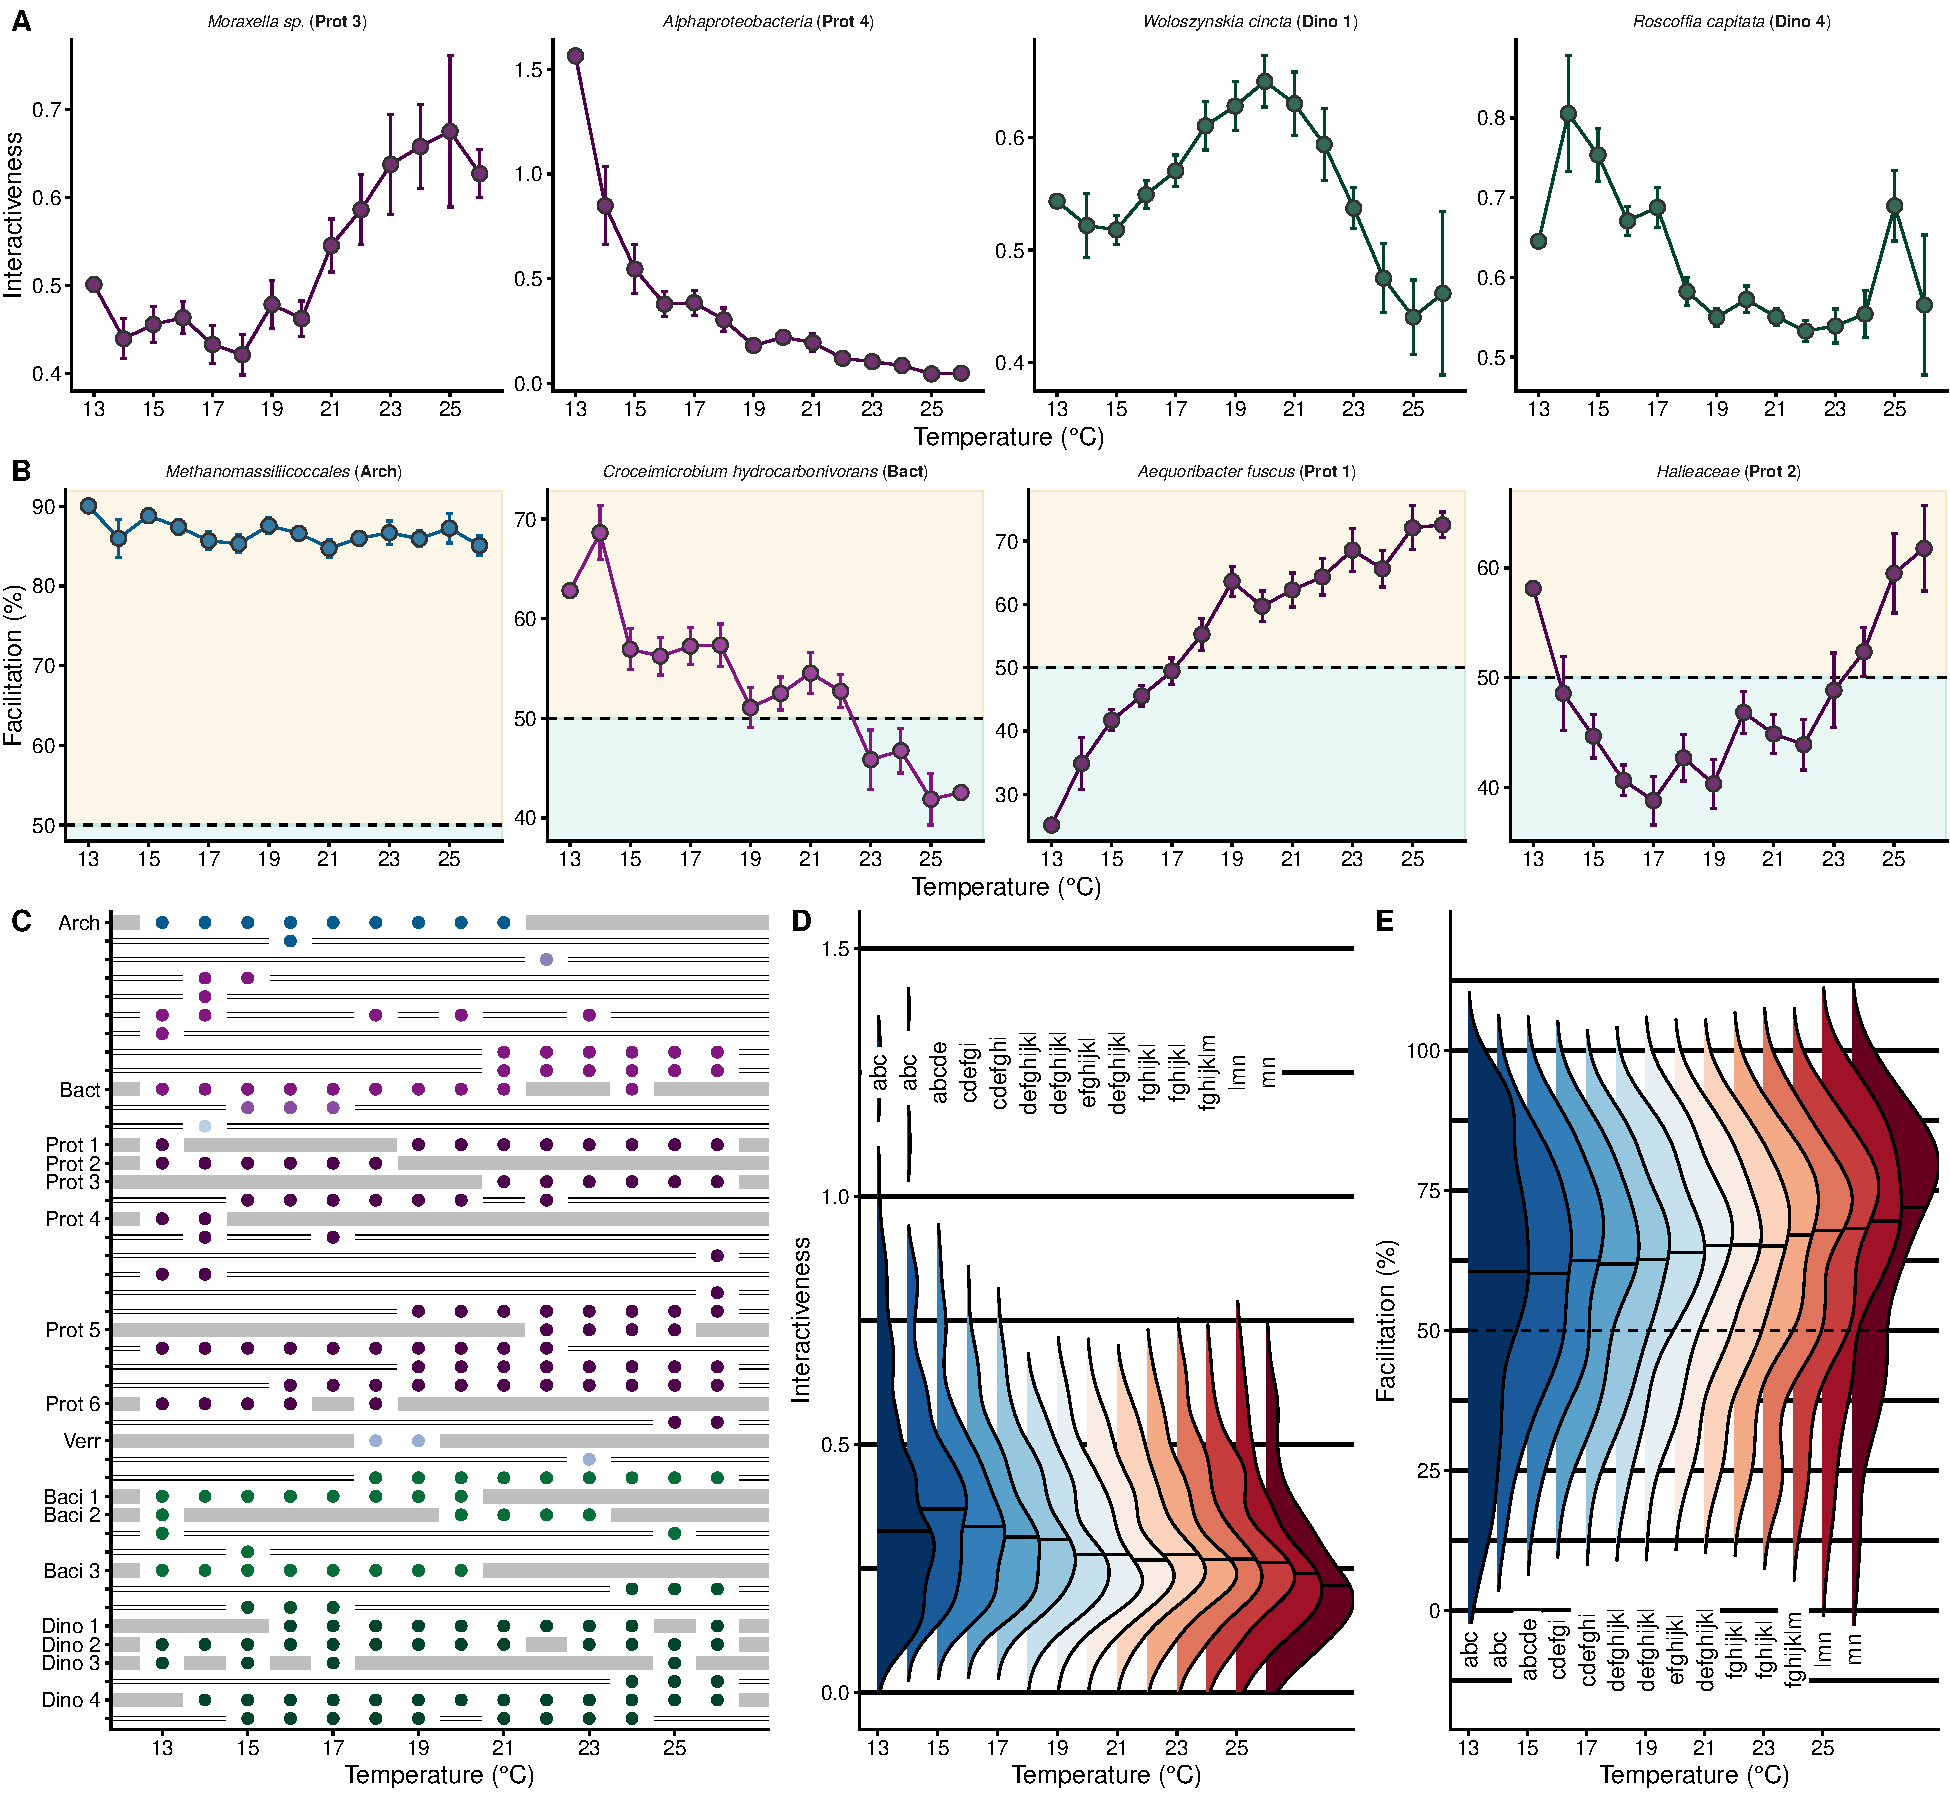
\includegraphics[keepaspectratio]{01-community-timeseries_files/figure-pdf/fig-4-temperature-dependency-1.pdf}}

}

\caption{\label{fig-4-temperature-dependency}图4：微生物互作网络随温度的动态变化综合面板}

\end{figure}%

\bookmarksetup{startatroot}

\chapter*{References}\label{references}
\addcontentsline{toc}{chapter}{References}

\markboth{References}{References}

\phantomsection\label{refs}




\end{document}
